\title{Determinants and the Area of a Parallelogram}
\subtitle{\SubTitleName}
\institute[]{\Course}
\author{\Instructor}
\maketitle   


\frame{\frametitle{Topics and Objectives}
\Emph{Topics} \\
\TopicStatement
\begin{itemize}

    \item relationships between area of a parallelogram and determinants
    
\end{itemize}

\vspace{0.5cm}

\Emph{Objectives}\\

\LearningObjectiveStatement

\begin{itemize}

    \item apply determinants to compute the area of a parallelogram

\end{itemize}

\vspace{0.25cm} 

}



\begin{frame}\frametitle{Area and Determinants}


    
    \begin{center}
    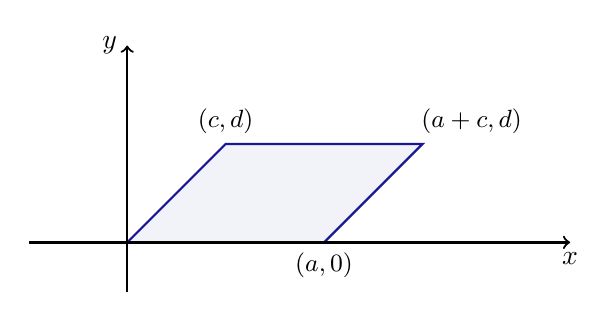
\begin{tikzpicture}[scale=1.25,thick]
        
        \onslide<2->{
        % boxes
        \filldraw[draw=DarkBlue!90,fill=DarkBlue!05] (0,0) -- (2,0) -- (3,1) -- (1,1) -- cycle; 
        \draw (1,1) node[above]{\small $(c,d)$};
        \draw (2,0) node[below]{\small $(a,0)$};
        \draw (3.5,1) node[above]{\small $(a+c,d)$};     
        \draw[->]  (-1,0) -- (4.5,0)  node [below] {$x$};
        \draw[->]  (0,-.5) -- (0,2)  node [left] {$y$};
        }
        
    \end{tikzpicture}
    \end{center}
    \onslide<3->{The area of a parallelogram is given by the formula}
    $$\onslide<4->{\text{area} = \text{base}\times\text{height} = a \times d}$$
    \onslide<5->{How might we use determinants to describe the area of a parallelogram?}

\end{frame}


\begin{frame}\frametitle{Area and Determinants}

    \begin{center}
    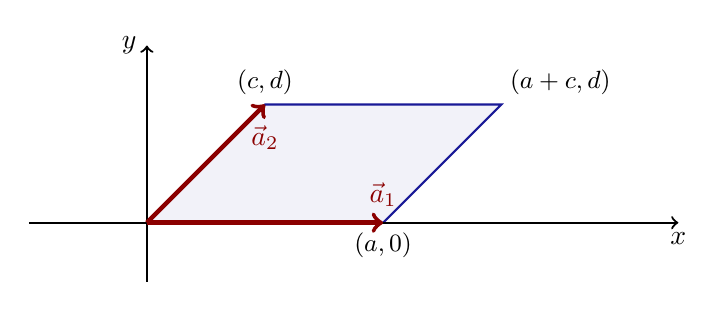
\begin{tikzpicture}[scale=1.5,thick]
        
        \onslide<2->{
        % boxes
        \filldraw[draw=DarkBlue!90,fill=DarkBlue!05] (0,0) -- (2,0) -- (3,1) -- (1,1) -- cycle; 
        \draw (1,1) node[above]{\small $(c,d)$};
        \draw (2,0) node[below]{\small $(a,0)$};
        \draw (3.5,1) node[above]{\small $(a+c,d)$};     
        \draw[->]  (-1,0) -- (4.5,0)  node [below] {$x$};
        \draw[->]  (0,-.5) -- (0,1.5)  node [left] {$y$};
        \draw[->,=>stealth,ultra thick,DarkRed]  (0,0) -- (2,0)  node [above=2pt,thick] {$\vec a_1$};
        \draw[->,=>stealth,ultra thick,DarkRed]  (0,0) -- (1,1)  node [below=4pt,thick] {$\vec a_2$};
        }
        
    \end{tikzpicture}
    \end{center}
    
    \onslide<2->{Constructing a matrix whose columns are $\vec a_1$ and $\vec a_2$ yields}
    \onslide<3->{$$A = \spalignmat{\vec a_1 \vec a_2}= \spalignmat{a c;0 d}, \quad \left| \det A \right| = | ad | = \text{area of parallelogram}$$}\onslide<4->{Also note that changing the value of $c$ (and keeping everything else constant) does not change the area of the parallelogram. }
\end{frame}



\begin{frame}\frametitle{More General Parallelograms}

    What if one side is not resting on a coordinate axes? Can we still use the determinant to give us the area of our parallelogram? 
    
    \vspace{12pt}
    \onslide<2->{
    Suppose we take the parallelogram we were using in the previous example, but rotate it about the origin by $\theta$ radians counter clockwise. The rotation will not change the area of the region. }
     
    \vspace{12pt}
    \begin{center}
    \begin{minipage}{.46\textwidth}
    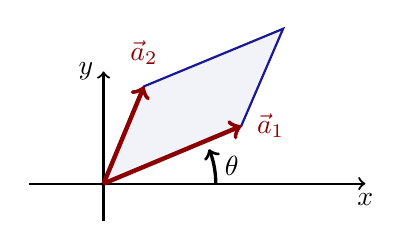
\begin{tikzpicture}[scale=0.95,thick]

        \coordinate (O) at (0,0);
        \coordinate (P) at (1.84,0.77);
        \coordinate (Q) at (2.4,2.07);    
        \coordinate (R) at (0.54,1.3);    
        
        \onslide<3->{
        % boxes
        \filldraw[draw=DarkBlue!90,fill=DarkBlue!05] (0,0) -- (P) -- (Q) -- (R) -- cycle; 
        % \draw (1,1) node[above]{\small $(c,d)$};
        % \draw (2,0) node[below]{\small $(a,0)$};
        % \draw (3.5,1) node[above]{\small $(a+c,d)$};     
        \draw[->]  (-1,0) -- (3.5,0)  node [below] {$x$};
        \draw[->]  (0,-.5) -- (0,1.5)  node [left] {$y$};
        \draw[black,->,=>stealth,very thick] (1.5,0) arc (0:22.5:1.2) node[midway, right] {$\theta$};  
        \onslide<4->{
        \draw[->,=>stealth,ultra thick,DarkRed]  (0,0) -- (P)  node [right=2pt,thick] {$\vec a_1$};
        \draw[->,=>stealth,ultra thick,DarkRed]  (0,0) -- (R)  node [above=4pt,thick] {$\vec a_2$};}
        }
        
    \end{tikzpicture}
    \end{minipage}\begin{minipage}{.5\textwidth}
    
    \onslide<5->{Will $|\det A| = |\det \spalignmat{\vec a_1 \vec a_2}|$ still give us the area of our parallelogram? }
    \end{minipage}
    \end{center}    
\end{frame}



\begin{frame}\frametitle{More General Parallelograms}

    If one side is not resting on a coordinate axes, will absolute value of the determinant still give us the area of our parallelogram? 
        
    \begin{itemize}
        \item<2-> Rotating the points that define our parallelogram by angle $\theta$ about the origin will not change the area of the parallelogram. 
        \item<3-> We can model a rotation of the points that define our parallelogram by multiplying $A$ with a rotation matrix. 
        $$A' = \spalignmat{\cos\theta, -\sin\theta;\sin\theta , \cos\theta} A = \spalignmat{\cos\theta ,-\sin\theta;\sin\theta , \cos\theta} \spalignmat{a c;0 d}$$
        \item<4-> Is the determinant of this new matrix also equal to $ad$? 
    \end{itemize}
    
\end{frame}



\begin{frame}\frametitle{More General Parallelograms}

    The determinant of a product of matrices is the product of the determinants.
    
    \pause 
    
    $$\det A' = \det \spalignmat{\cos\theta, -\sin\theta;\sin\theta ,  \cos\theta} \det \spalignmat{a c;0 d} = (1) \, (ad) = ad $$
    
    \pause 
    \vspace{12pt}
    
    \begin{center}\begin{tikzpicture} \node [mybox](box){\begin{minipage}{0.80\textwidth} \vspace{4pt}

        The absolute value of the determinant of a $2\times 2$ matrix, whose columns  determine adjacent edges of a parallelogram, will give the area of the parallelogram. 

    \end{minipage}}; \node[fancytitle, right=10pt] at (box.north west) {Theorem}; \end{tikzpicture}\end{center}
 



\end{frame}


\begin{frame}\frametitle{Example: Area of a Parallelogram}

    Compute the area of the parallelogram determined by $ \vec 0, \vec u, \vec v$, and $\vec u + \vec v$, where 
    \begin{equation*}
    \vec u = \begin{pmatrix*}[r]
        -1 \\ 2 
    \end{pmatrix*} \quad 
        \vec v = \begin{pmatrix*}[r]
        3 \\ 1 
    \end{pmatrix*} 
    \end{equation*}
    
    \onslide<2->{ 
    \Emph{Solution}
    }
        \begin{center}
        \begin{minipage}{.57\textwidth}
    \onslide<3->{The absolute value of the determinant of a matrix whose columns are $\vec u$ and $\vec v$ yields \begin{align*}
        \text{area} &= |\det A| \\ &= \left| \det \spalignmat{-1 3; 2 1}\right| \\ &= | -1 -6 |=7 
    \end{align*}}
    \end{minipage}\begin{minipage}{.42\textwidth}
    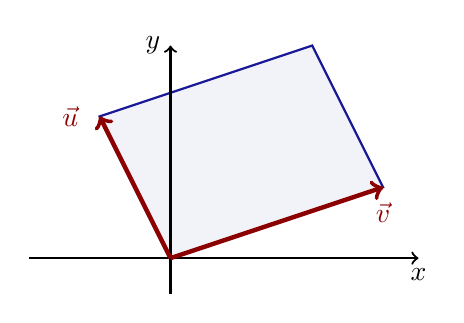
\begin{tikzpicture}[scale=0.9,thick]

        \coordinate (O) at (0,0);
        \coordinate (P) at (3,1);
        \coordinate (Q) at (2,3);    
        \coordinate (R) at (-1,2);    
        
        \onslide<3->{
        % boxes
        \filldraw[draw=DarkBlue!90,fill=DarkBlue!05] (0,0) -- (P) -- (Q) -- (R) -- cycle; 
        % \draw (P) node[right]{\small $(3,1)$};
        % \draw (R) node[above=2pt]{\small $(-1,2)$};
        % \draw (3.5,1) node[above]{\small $(a+c,d)$};     
        \draw[->]  (-2,0) -- (3.5,0)  node [below] {$x$};
        \draw[->]  (0,-.5) -- (0,3)  node [left] {$y$};
        \onslide<3->{
        \draw[->,=>stealth,ultra thick,DarkRed]  (0,0) -- (P)  node [below=2pt,thick] {$\vec v$};
        \draw[->,=>stealth,ultra thick,DarkRed]  (0,0) -- (R)  node [left=4pt,thick] {$\vec u$};}
        }
        
    \end{tikzpicture}
    \end{minipage}
    \end{center}    

\end{frame}



\frame{\frametitle{Summary}

    \SummaryLine \vspace{4pt}
    \begin{itemize}\setlength{\itemsep}{8pt}
        \item the use of determinants to compute the area of a parallelogram
    \end{itemize}
    % A convenient method for computing the area of a parallelogram has applications in 
}


